\documentclass{beamer}

\mode<presentation>
{
  \usetheme{Warsaw}
  \usecolortheme{seahorse}
  \setbeamercovered{transparent}
}

\usepackage[english]{babel}
\usepackage[latin1]{inputenc}
\usepackage{times}
\usepackage[T1]{fontenc}
\usepackage{graphicx}

\title{My Uml Paper}
\subtitle{How To Write Papers With Uml}
\author[Me]{Me Myself \ \texttt{me@myself.edu}}
\date[UML2015]{How To Make A Beamer With Plant Uml Pictures}
\subject{Plant Uml}

\begin{document}

\begin{frame}
  \titlepage
\end{frame}

\begin{frame}
  \tableofcontents
\end{frame}

\section{First steps}

\begin{frame}{How to itemize}
      \begin{itemize}
          \item Approach one.
          \begin{itemize}
            \item First dot.
            \item Another.
        \end{itemize}
          \item Approach two.
          \begin{itemize}
            \item First dot. First dot. First dot.
                  \\* Long one. Long one.
            \item Another.
                  \\* Long one.
                  \\* Even more.
        \end{itemize}
    \end{itemize}
\end{frame}

\begin{frame}[fragile]{How to verbatimize}
    \begin{columns}
        \column{.5\textwidth}
            This program \texttt{return}s 0.
\begin{verbatim}
int main()
{
    return 0;
}
\end{verbatim}
        \column{.5\textwidth}
            This program \texttt{return}s 1.
\begin{verbatim}
int main()
{
    return 1;
}
\end{verbatim}
    \end{columns}
\end{frame}

\begin{frame}[fragile]{Putting large portion of code}
\tiny
\begin{verbatim}
struct Keeper
{
    Keeper(int keeping, int keptout);

    void doing();
    int done();
    const Keeper& didnt() const;

private:
    int kept_;
};

struct Another
{
    typedef Keeper the_keeper;

    int one;
    int two;
    int three;
};
\end{verbatim}
\end{frame}

\section{Graphics}

\begin{frame}{Sequence Diagram}
    \begin{columns}
        \column{.5\textwidth}
            \includegraphics[scale=0.6]{build/sequence1.eps}
        \column{.5\textwidth}
            \includegraphics[scale=0.6]{build/sequence2.eps}
    \end{columns}
\end{frame}

\begin{frame}{Arbitrary Diagram}
    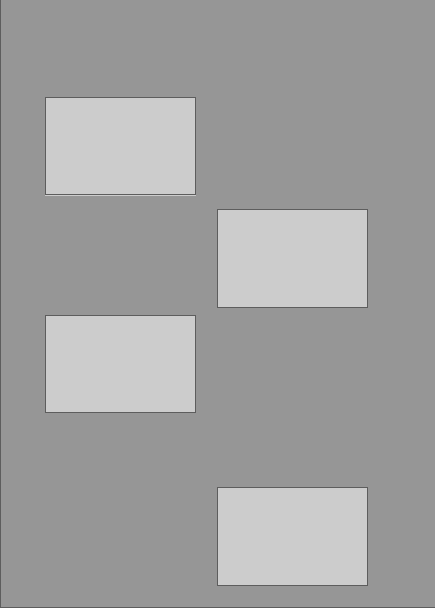
\includegraphics[scale=0.6]{build/diagram.pdf}
\end{frame}

\section{Things missing}

\begin{frame}
    \begin{itemize}
        \item Automate exporting libre drawing.
        \item How to import code from file?
        \item How to align and size pictures?
        \item How to draw vector graphics?
    \end{itemize}
\end{frame}

\end{document}
